
\section{Overview of LLM-QO}
\label{sec:overview}

\begin{figure*}
  \centering
  %\includegraphics[width=0.85\textwidth]{figures/figure1.pdf}
  \includegraphics[width=1\textwidth]{figures/alloverview_llmqo.pdf}
  \caption{The overview of \LLMQO, which consists of: (a) \QueryInstruct and the data preparing pipeline,  (b)The training pipeline for LLMs, and (c) The inference pipeline.
 % The \QueryInstruct pipeline is responsible for formulating the prompt of \LLMQO and constructing instruction data and preference data for two training stages. The training pipeline of \LLMQO is composed of two stages: Query Instruction Tuning(\QIT) and Query Direct Preference Optimization(\QDPO). During the inference stage, the tuned LLM takes the the raw text of the input query, corresponding statistics involved by the query, and a one-shot demonstration as input and generate the execution plan.
  }
  \label{fig:pipline}
\end{figure*}

We present the overview of our approach, \LLMQO, whose framework is illustrated in Fig.~\ref{fig:pipline}.
\LLMQO comprises two main pipelines, a data preparing pipeline and a training pipeline for LLMs. 

The data preparation pipeline is a crucial initial step in \LLMQO. It generates the training data regarding a data recipe, named \QueryInstruct, which will be used to fine-tune the LLM in the training pipeline.
For data preparation, the gist of designing \QueryInstruct is to keep the data informative and concise, so that feeding an LLM with sufficient instructions and knowledge while saving token usage.
%In the data preparing pipeline, LLM-QO generates the data recipe, \QueryInstruct, given a set of training queries, which is used for training an LLM in the training pipeline.
Serving as the foundation of \LLMQO training, \QueryInstruct includes five elements as follows: \ding{172} Query: the SQL query that needs optimization. 
\ding{173} Instruction of query optimization: guidelines and instructions on how to optimize the given queries and explanations of the input.
\ding{174} Auxiliary information: including the database schema and relevant statistics that provide context and support for query optimization.
\ding{175} High-quality plans: efficient execution plans of the query that are serialized and converted into a textural format. 
\ding{176} Planning demonstration: one concrete planning example to alleviate the hallucination of the LLM.
It is worth noting that the query, instruction, auxiliary information, and demonstration compose the prompt of the LLM, and the textualized execution plan is the target response used for model fine-tuning. 
Given a query workload, the execution plans can be collected from traditional query optimizers, especially the optimizers of commercial DBMS, which have been delicately designed over decades. 
%The gist of \QueryInstruct design is to keep the data informative and concise, so that feeding LLM with necessary instructions and knowledge while saving the volume of tokens. 
%Analogy to user prompt, the data recipe contains the query itself, the instruction of query optimization and auxiliary information such as the statistics and the schema of the database. Furthermore, to steer LLM towards inferring valid and efficient execution plan, the data recipe also contain high-quality plans, which is serialized and texturalized to enable sequence-to-sequence generation. 
We will elaborate on the construction of \QueryInstruct in ~\cref{sec:method:queryinstruct}. 

The LLM training pipeline is designed to fine-tune an LLM with the training data from a query workload, which is generated regarding \QueryInstruct in the first pipeline. Considering the intrinsic difficulty of the problem, we adopt a two-stage training workflow to gradually enhance the reasoning capability of an LLM for query planning.
% In the training pipeline, we propose a two-stage training workflow based on the data recipe \QueryInstruct. 
The first stage initiates an LLM the ability to generate an execution plan for a given query by Instruction Tuning. This stage mainly aims at bootstrapping a general-purpose LLM to generate accessible and valid plans. 
Subsequently, the second stage further improves the planning capability of an LLM by training it to 
distinguish a good plan from ordinary plans.
%distinguish an ordinary plan between good plan. 
Through this stage, the LLM is expected to infer efficient execution plans. 
In a nutshell,  this two-stage training workflow guides the LLM to distill and synthesize the behavior of multiple query optimizers, in a parameterized fashion, so that earn the potential of being an overall best optimizer. We will delve into the training pipeline of \LLMQO in ~\cref{sec:method:training}.

In inference stage, as shown in Fig.~\ref{fig:pipline}(c), a test query and corresponding auxiliary information are inserted into an input prompt, following the formulation of \QueryInstruct. Afterwards, an  inference calling is issued on the fine-tuned LLM, by feeding the  prompt into the model and obtaining the response. Finally, the textual response is transformed into an execution plan for query  evaluation.

% We employ cost-based optimizers such as Oracle and PostgreSQL to select optimal query execution plans. 
% Additionally, we introduce perturbations to the optimizer, utilizing methods such as hint-based adjustments and cardinality estimation techniques, to further refine plan selection.
% In the initial phase of our approach, we rely exclusively on plans generated by Oracle and PostgreSQL to ensure that the model produces valid plans with performance comparable to PostgreSQL. In the subsequent phase, we execute plans generated under various perturbation strategies applied to the cost-based optimizer, selecting faster plans as positive samples and slower plans as negative samples. This method leverages the strengths of both traditional cost-based optimization and innovative perturbation techniques to enhance query performance and robustness.

\section{Formulation of \QueryInstruct}
\label{sec:method:queryinstruct}
We first introduce the formulation of our data recipe, \QueryInstruct, followed by the procedure of  training data collection. 

\begin{figure}[t]
\centering
\begin{subfigure}[Physical Plan]{%
\scriptsize  % \footnotesize
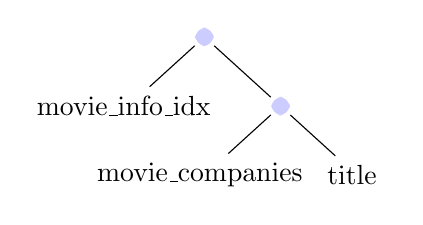
\begin{tikzpicture}[sibling distance=5.5em, level distance = 2.5em,
  every node/.style = { shape= rectangle, rounded corners,
    draw =none , align=center,
   % top color=white, bottom color=blue!20
   }]]
  \node[fill=blue!20] { \HashJoin } 
      child {
        node { movie\_info\_idx }
      }
      child {
        node[fill=blue!20] { \HashJoin }
          child { node{ movie\_companies } }
          child {
              node { title }
                }
            }
  ;
\end{tikzpicture}
 % }
  \label{fig:example:plan}
}\end{subfigure}
\begin{subfigure}[The Planning Path]{%
%  \includegraphics[width=0.66\columnwidth,height=2.2cm]{
\scriptsize  %\footnotesize %
% \resizebox{0.25\textwidth }{!}{%
\begin{tabular}{m{0.6cm} p{4.0cm}}
\toprule
Step1: & [movie\_companies, title, \HashJoin] \\
% Step 2: & [ movie\_info\_idx, Step 1, \HashJoin] \\
Step2: & [movie\_info\_idx, \HashJoin(movie\_companies title), \HashJoin] \\
 \bottomrule
\end{tabular}
  \label{fig:example:planpath}
}\end{subfigure}
%
\begin{subfigure}[The Bracket Sequence]{%
%  \includegraphics[width=0.66\columnwidth,height=2.2cm]{
\scriptsize  %\footnotesize %
\begin{tabular}{c l}
\toprule
\HashJoin(movie\_info\_idx \HashJoin(movie\_companies title)) \\ 
\bottomrule

\end{tabular}
  \label{fig:example:bracket_sequence}
}\end{subfigure}
\caption{A plan with two textual representations}
\label{fig:example}
\end{figure}

\begin{figure}
    \centering
    \footnotesize
    \begin{subfigure}{}
        \centering
        %\label{fig:query_instruct:prompt}
        %\resizebox{!}{0.5\textwidth}{
        %\resizebox{0.5\textwidth}{!}{
        \begin{tcolorbox}[colback=yellow!10!white, colframe=blue!75!black]
            \textbf{INSTRUCTION:} You are a SQL query optimizer. You will be given a multi-table SQL query {\color{Orchid} \texttt{<SQL>}} and the statistics of the tables involved in the query {\color{BlueGreen} \texttt{<Statistics>}}. The statistics include the minimum value, maximum value, and the count of distinct values for each column of each table in the query, in the format of [min, max, distinct count]. Your task is to generate the optimal execution plan for the given SQL query. You should represent the execution plan using a bracket sequence, where \HashJoin, \NestLoop, or \MergeJoin are used to join the tables in the SQL query. Let's think step by step and show your reasoning before showing the final result. {\color{Peach} \texttt{<Planning Demonstration>}: \texttt{<SQL>}: ..., \texttt{<Statistics>}:..., \texttt{<Response>}:...}
            
            \textbf{INPUT:}
            \begin{Verbatim}[commandchars=\\\{\}]
\textcolor{Orchid}{<SQL>}: \textcolor{blue}{SELECT} * \textcolor{blue}{FROM} movie_companies, title, movie_info_idx  
\textcolor{blue}{WHERE} title.movie_id = movie_companies.movie_id \textcolor{blue}{AND} 
title.movie_id = movie_info_idx.movie_id  \textcolor{blue}{AND} 
movie_companies.company_type_id = 1 \textcolor{blue}{AND} 
title.product_year < 1904 \textcolor{blue}{AND} title.product_year > 58;
\textcolor{BlueGreen}{<Statistics>}: 
title (movie_id: [0,2527968,2527969], kind_id: [-1,7,7], 
product_year: [-1,2019,134], imdb_id: [-1,2012,10]), 
movie_companies (movie_id: [-1,2525401,1087136], 
company_id: [1,234997,234997], company_type_id: [1,2,2]), 
movie_info_idx (movie_info_idx_id: [0,1380033,1380034], 
movie_id: [-1,2525449,459876]).
            \end{Verbatim}          
        \end{tcolorbox} 
        %}
        \label{fig:query_instruct:prompt}
    \end{subfigure}%
    
    \vspace{-3ex}
    \begin{subfigure}{}
        \centering
        %\caption{[The Response]}
        \label{fig:query_instruct:response}
        \begin{tcolorbox}[colback=yellow!10!white, colframe=blue!75!black]
            \textbf{RESPONSE:}\\
            Step1: [movie\_companies, title, \HashJoin], \\
            Step2: [movie\_info\_idx, \HashJoin(movie\_companies title), \HashJoin], \\
            % Step2: [movie\_info\_idx, Step1, \HashJoin],\\
            Therefore, the final answer is: \\ \HashJoin (movie\_info\_idx \HashJoin(movie\_companies itle)).
        \end{tcolorbox}
        \label{fig:query_instruct:response}
    \end{subfigure}
%    \vspace{0.2cm}
    \caption{The format of \QueryInstruct}
    \label{fig:query_instruct} % 添加整体图形标签
\end{figure}

\subsection{\QueryInstruct Preparation}
\label{sec:method:query_instruct:prepare}
%In the pursuit of enhancing LLMs’ capabilities to tackle the query optimization problem with explicit reasoning paths, we develop a new dataset named QueryInstruct. 
For a SQL query in the training workload, \LLMQO generates its data recipe for the two-stage training, which is conducted offline.
%which is offline regarding the training procedure. 
To start with, we present the formulation of the prompt of \LLMQO, which is composed of the input prompt and a response, as shown in Fig.~\ref{fig:query_instruct}. 
%For each SQL query $q$, LLM-QO generates a data recipe including textual representation of the instruction $x$, the input query $q$ and the serialized planing path $p$.

%\subsubsection{Prompt Templates for LLM-QO}
%\label{prompt_templates}
%task description 
%meta information
%SQL query
%=> Output plan
\stitle{Prompt Design.}
The prompt, as a user-specific input of LLM, includes a query, the instruction, the auxiliary information and a planning demonstration.
%Prompts refer to user-generated inputs, including queries, instructions, or questions, that steer large language models and dictate their behavior for particular tasks. In this paper, we design the following prompt template to train and generate output for the query optimization task using the Llama models. We give the instruction, input, and response to the LLMs during training. When testing, we only provide the instruction, and input, and ask the LLMs to generate the response.
Fig.~\ref{fig:query_instruct} illustrates the input prompt of \LLMQO, for both training and inference. The first part of the prompt is the instruction that requires the LLM to mimic as a SQL query optimizer. 
There are two placeholders, {\color{Orchid}\texttt{<SQL>}} and {\color{BlueGreen} \texttt{<Statistics>}}, indicating the raw text of the input query and corresponding statistics involved by the query.  
The contents of these two placeholders are attached below the prompt template. 
Specifically, to help LLM understand the semantics of the statistics, the prompt concisely describes the per-column statistics in a bracket format. In addition, we specify the plan output in a sequence of bracket representation, which we will introduce later, as well as the the join operators supported in the system. 
%For SQL query planning, we design the prompt of LLM as shown in Fig.~\ref{fig:query_instruct}. 
%The prompt contains the instruction of query optimization, the raw-text of SQL query \texttt{<SQL>} and the statistics of \texttt{<Statistics>} involved the query. Specifically, we request the LLM to mimic a query optimizer, by declaring the available physical operators. 
To initiate the reasoning capability of LLM, we encourage the LLM to generate a plan by  explicit instruction `think step by step'~\cite{DBLP:conf/nips/KojimaGRMI22}. 
Considering different LLMs support different maximum length of input tokens, users can further enrich the database statistics, e.g., the histograms, distinct values, estimated 
cardinalities, etc, which are available in the database catalog. 

At the end of the instruction, we add a one-shot planning demonstration identified by a placeholder {\color{Peach}\texttt{<Planning Demonstration>}} as shown in Fig.~\ref{fig:query_instruct}. 
It is challenging for general LLMs to consistently generate valid plans as users can issue any syntactically correct queries. In our extensive trials, LLMs tend to infer invalid plans when the involved tables and columns are unseen in the training queries. Therefore, we further introduce in-context learning into the prompt design to alleviate invalidation, which is also used in table understanding~\cite{DBLP:journals/pacmmod/LiHYCGZF0C24} and query rewriting~\cite{DBLP:journals/corr/abs-2404-12872} tasks.
%
Here, a planning demonstration serves as an illustrative example to align LLM to our query optimization task.
The demonstration is assembled by an exemplar {\color{Peach}\texttt{<SQL>}}, the pertinent statistical information {\color{Peach}\texttt{<Statistics>}}, and the output plan of the exemplar query {\color{Peach}\texttt{<Response>}}.
To avoid invalid generation to the largest extent, we plug an exemplar query into the demonstration, which possesses the same query template, i.e., the same set of tables and join conditions, as the input query. 
At the current stage, that is the most effective strategy in our extensive attempts on various test queries from multiple workloads. 
It is worth noting that the plans in the response are unnecessary to be well performed. We find that LLMs only refer to the occurrence of tables and columns, and will generate a new plan in most cases. 


\stitle{Response Generation.}
The curial design of \QueryInstruct is to represent the tree-shape execution plan as a textual sequence, which preserves the intact execution strategy, i.e., the join order and the physical operators for LLMs to comprehend. 
A straightforward way is to represent the plan in a bracket format. For instance, Fig.~\ref{fig:example:bracket_sequence} presents the bracket representation of the query plan in Fig.~\ref{fig:example:plan}, where the bracketed tokens $opt(opd_1, opd_2)$ denote a join operation $opt$ on a left sub-plan and a right sub-plan. 
The sub-plans $opd_1, opd_2$ are either base table names or nested bracket representations. 
Although the bracket representation consumes minimal tokens, it fails to stimulate the multi-step reasoning capability of LLMs in the context of query optimization.
%, the sequential representation should also stimulate the multi-step reasoning capability of LLM in the context of query optimization, 
%The data recipe, QueryInstruct, also contains the model's target prediction of two-stage training workflow, i.e., one or multiple execution plans of a training query $q$. As Fig.~\ref{fig:pipline} depicted, we inject the SQL queries into multiple DBMSs, e.g, PostgreSQL, Oracle, DB2, and obtain the real execution plans output by their query optimizers.
%
To this end, we devise a structured hierarchical representation, planning path, for an execution plan $p$. For a query involving $n$ tables, its planning path comprises $n - 1$ sequential steps $[s_1, s_2, \cdots, s_{n-1}]$ where each step $s_i$ denotes one non-leaf (join) operator. We use a sequence of tokens $s = [ opd_1, opd_2, opt ]$ to represent one step, where $opd_1$, $opd_2$ are either base table name or intermediate step and $opt$ is the name of the physical operator.  
The order of the steps in the planning path is determined by the post-order traversal of the tree-shape execution plan, which also aligns with the bottom-up query execution semantic.
As an example, Fig.~\ref{fig:example:planpath} demonstrates the corresponding planning path for the query in Fig.~\ref{fig:example:plan}. 
The complete response includes the planning path as reasoning steps and the bracket representation as the final answer as shown in Fig.~\ref{fig:query_instruct}. 
\LLMQO will transform the response into an execution plan for query execution.


\subsection{Training Data Preparation}
\label{sec:queryinstruct:PDG}
Formulated by the data recipe \QueryInstruct, \LLMQO prepares the training data from a query workload of a database instance. 
In the two-stage training pipeline, 
we use instruction data $(\bm{x}, \bm{y})$ and preference data $(\bm{x}, \bm{y}_{w}, \bm{y}_{l})$ to train the model by Query Instruction Tuning in the first stage and Query Direct Preference Optimization in the second stage, respectively, where $\bm{x}$ denotes the input prompt of a query, 
%y第一次出现 但是缺乏解释;y是SFT阶段的ground truth
%Figure1的y字体和latex的字体不太对应
$\bm{y}, \bm{y}_{w}, \bm{y}_{l}$ denote expected responses of LLM. 
In particular, for the preference data, $\bm{y}_{w}$ contains a well-performed execution plan and $\bm{y}_{l}$ contains an ordinary plan by contrast, for a same query in $\bm{x}$, reflecting a planning preference we wish the LLM to absorb and deliver. 
We concentrate on the preparation of the training data and defer the technical details of our training algorithms to~\cref{sec:method:training}.


\stitle{Execution Plan Collection.} As training data, original execution plans can be collected from existing query optimizers, which are available in query logs. As Fig.~\ref{fig:pipline} depicts, \LLMQO collects execution plans from multiple DBMSs, e.g., \Postgres, \Oracle, based on the real performance of the execution plans. 
It is worth mentioning that we also tried using the cost of the plan, derived from traditional cost models, as the evaluation metric for selecting training plans. However, as is well-known, the real performance of execution plans is inconsistent with their cost, which compromises the efficiency of plans generated by LLMs.

\begin{algorithm}[t]
	%\footnotesize
	\small
    \caption{Preference Data Generation}
	\label{alg:pdg}
	\DontPrintSemicolon
    \SetKwData{Procedure}{Procedure}
	\SetKwData{Up}{up}  \SetKwInOut{Input}{Input} \SetKwInOut{Output}{Output}
    \SetKwInOut{Initialize}{Initialize}
    
	\Input{SQL query $q$, $k$ optimizers,  threshold $r_0$}

	\Output{$\mathbb{D}_{\mathrm{dpo}}$ of $q$}

    Initialize $\mathbb{D}_{\mathrm{dpo}} \leftarrow \emptyset$, $p^* \leftarrow \varnothing$, $t^* \leftarrow \infty$\;
    \For{$ i \leftarrow 1$ to $k$}{
    \label{line:plan_and_time:start}  
        generate plan $p_i$ by the $i$-th optimizer \;
        obtain the execution time $t_i$ of $p_i$ in the execution engine \;
        \If {$t_i < t^*$}{ \label{line:plan_compare}
            $p^* \leftarrow p_i$, $t^* \leftarrow t_i$\;
        }
    } \label{line:plan_and_time:end}  
    generate input $\bm{x}$ for $q$ and output $\bm{y}_w$ for $p^{*}$ as Fig.~\ref{fig:query_instruct} \; \label{line:prompt_generate}
    %generate output $\bm{y}_w$ for $p^{*}$ \; \label{line:prefer_response_generate}
        
        \For{$ i \leftarrow 1$ to $k$}{
    \label{line:data_collection:start}
        % \For{$j \leftarrow i + 1 $ to $k$}{
            % \If {$t_*/t_j < r_0$}{
            \If {${t^{*}}/{t_i} < r_0$}{ \label{line:gap_compute}
                generate output $\bm{y}_l$ for $p_i$\;
                add ($\bm{x}$, $\bm{y}_w$, $\bm{y}_l$) into $\mathbb{D}_{\mathrm{dpo}}$ \;
                }
        }\label{line:data_collection:end}
    % }
\Return{$\mathbb{D}_\mathrm{dpo}$} \;
\end{algorithm}

\stitle{Preference Plan Generation.}
To obtain a pair of preferred and dispreferred plans, \LLMQO collects the execution plans from multiple query optimizers of different DBMSs and selects those plans with a performance gap. 
%In this section, we aim to create a synthetic preference pair dataset for the DPO stage utilizing SQL queries and their corresponding actual execution plans from various DBMSs. 
For one query $q$ in a training workload, the procedure for generating preference data is detailed in Algorithm~\ref{alg:pdg}.
% Algorithm~\ref{alg:pdg} presents the preference data generation process in \QueryInstruct. 
Given $k$ optimizers, first, we collect the $k$ corresponding plans $\{p_1, \cdots, p_k\}$ and obtain the execution time of plan $p_i$ in a certain execution engine, denoted as $t_i$ (line~\ref{line:plan_and_time:start}-\ref{line:plan_and_time:end}). Here, the optimal plan $p^*$ with a minimum execution time $t^*$ is chosen as the preferred plan in $\bm{y}_w$ (line~\ref{line:plan_compare}-\ref{line:plan_and_time:end}).   
Subsequently, we generate the prompt for the query and the preferred response $\bm{y}_w$ for $p^*$ (line~\ref{line:prompt_generate}).
Finally, we compare the performance of others' plans with $p^*$. If $t^*/t_{i}$ is smaller than a threshold $r_{0} \in (0, 1)$, we choose plan $p_i$ as a dispreferred plan and generate its response $\bm{y}_l$ (line~\ref{line:data_collection:start}-\ref{line:data_collection:end}). 
In this procedure, we keep a single preferred plan $p^*$, instead of selecting preferred and dispreferred plans from round-robin tournaments. 
This will result in a simpler decision-comparing task, making the model performance in the second-stage training more stable.
It is worth mentioning that when additional query optimizers are available, the preference data set $\mathbb{D}_{\mathrm{dpo}}$ can be extended incrementally for $q$. We can extend Algorithm~\ref{alg:pdg} to collect the plan preference pairs between the additional query optimizer and existing $k$ optimizers. Specifically, we add pairs of plans where the optimal plan $p^*$ is from the new optimizer (line~\ref{line:prompt_generate}). 
The new optimizer is expected to further compensate for the unsatisfactory performance of existing $k$ optimizers on some queries, thereby enhancing the overall performance of \LLMQO.



\section{Training of \LLMQO}
\label{sec:method:training}
Based on the data recipe \QueryInstruct, we develop a fine-tuning pipeline in \LLMQO to enhance the capability of general-purpose LLMs in dealing with  query optimization tasks. 
Our fine-tuning strategy for \LLMQO is composed of two stages, as illustrated in Fig.~\ref{fig:pipline}.
To be more specific, the first stage, called Query Instruction Tuning (\QIT), focuses on initiating LLMs into interpreting and resolving the query optimization task by imitating generic query optimizers, which aims at empowering LLMs to generate valid plans. 
%Specifically, the first stage focuses on refining the model's ability to interpret and resolve query optimization problem through Instruction Tuning. 
The second stage, named as Query Direct Preference Optimization (\QDPO), further enhances the model's proficiency as an intelligent query planner by training it to differentiate between good and plain execution plans.
Both of the two stages are implemented by efficient fine-tuning technique LoRA. 
%
%The first stage equips the model with the capability to generate valid plans. Building on this foundation, the second stage trains the model to differentiate between more efficient and less efficient planning paths, thereby improving its capacity to produce efficient execution plans.
We will present the algorithmic details in this section.

\subsection{Query Instruction Tuning}

The first stage of our training, called Query Instruction Tuning
(\QIT), takes the prompt $\bm{x}$ as input and guides LLMs to infer its corresponding plan $\bm{y}$ as output, which includes the planning path and the bracket final answer. 
\QIT conducts supervised fine-tuning (SFT) on a pre-trained LLM $\pi$ using a training query set $\mathbb{D}_{\mathrm{sft}}$. 
Let $\pi(\bm{y} \mid \bm{x})$ denote the predictive conditional probability computed by Eq.~\eqref{eq:cond_prob}. This stage minimizes the negative log-likelihood as shown in Eq.~\eqref{eq:sft_loss} using stochastic gradient descent, which is consistent with Eq.~\eqref{eq:mle_loss}. 
%This training step equips the LLMs with the ability to generate a valid execution plan for a SQL query by following query optimization task instructions.
% \kfadd{Imitation learning: AlphaGo~\cite{silver2016mastering}}
% During this stage, we employ supervised fine-tuning (SFT) on a pre-trained LLM, $\pi$, using a dataset $\mathbb{D}_{\mathrm{sft}}$
% consisting of high-quality query instruction and response pairs. 
% The LLM model is trained to take the task description, SQL query, and schema statistics as input $x$ and to generate the textual planning path $y$ as output. Starting from a base LLM $\pi$, SFT maximizes the likelihood of response $y$ given prompt $x$
% as defined in the Eq.~\eqref{eq:sft_loss}.
\begin{align}
    \label{eq:sft_loss}
    \mathcal{L}_{\mathrm{sft}}({\theta}) = \mathop{\mathbb{E}}_{( \bm{x}, \bm{y}) \sim \mathbb{D}_{\mathrm{sft}}} -\Big[ \log \pi(\bm{y} \mid \bm{x})\Big]\text{.}
\end{align}
\QIT is intrinsically supervised imitation learning~\cite{DBLP:journals/csur/HusseinGEJ17} that is a widely-used bootstrap strategy for building complicated agents from scratch.  
For example, the intelligent Go player AlphaGo~\cite{silver2016mastering} learns from a large number of expert game records through supervised learning and then improves its self-play ability through reinforcement learning.
For the query optimization task, the expert experiences are collected from well-designed query optimizers. 
For an input query in $\bm{x}$, \QueryInstruct encapsulates its best plan in $\bm{y}$ among $k$ optimizers. 
Thereby, in the first stage of training, \LLMQO not only learns to resolve the query optimization task step-by-step, but also `distills' the overall best optimizer among the $k$ experts. 
%The seq2seq models are trained using a teacher forcing mechanism, in which the actual ground truth tokens are supplied during training to minimize the loss function specified in Eq.~\eqref{eq:sft_loss}.
%This optimization process trains the model to map SQL queries and the textual prompts to their corresponding planning paths, thereby fostering a deep understanding of how to navigate and solve the query optimization task using step-by-step reasoning. 
%The model developed in Stage 1 is named $\pi_{\textnormal{sft}}$.

% \COMMENT{The SFT loss is computed based on the discrepancy between the model’s predicted planning paths and the actual planning paths in the dataset, formally defined as follows:}

% %maximize the probability the model will
% re-produce similar gold standard responses. In many ways SFT is simply training the
% model to mimic the gold standard responses.




\comment{
\begin{algorithm}[t]
	%\footnotesize
	\small
    \caption{Preference Data Generation}
	\label{alg:pdg}
	\DontPrintSemicolon
    \SetKwData{Procedure}{Procedure}
	\SetKwData{Up}{up}  \SetKwInOut{Input}{Input} \SetKwInOut{Output}{Output}
    \SetKwInOut{Initialize}{Initialize}
	\Input{query prompt set $\{x_1, \ldots, x_n\}$, execution Engine $E$, threshold for preference data selection $r_0$}

	\Output{preference data $\mathbb{D}_{\mathrm{dpo}}$}
    
	\SetKwFunction{Emit}{Emit}
	\SetKwFunction{Check}{Check}
       
	\For{$i \leftarrow 1$ to $n$}{ 
        $(y_{i1}, \ldots, y_{ik})$ ;
     \algocomment{generate $k$ plans from DBMSs for prompt $x_i$} \;

    $(r_{i1}, \ldots, r_{ik}) \,|\, r_{ij} = E(x_i, y_{ij})$ ;
    \algocomment{obtain execution time for each plan}
    
        \For { $j \leftarrow 1$ to $k$ } 
        {
        \For { $l \leftarrow 1$ to $k$ } 
        {
        \If {$j == l$}{
          $continue$ ;
          }
        $r \leftarrow r_{ij}/r_{il}$ ;
        \algocomment{compute the speed-up ratio between the pair of plans $y_{ij}$ and $y_{il}$} \;
        \If{$r > r_0$~}{
        $\mathbb{D_{\text{pref}}} \leftarrow \{\mathbb{D_{\text{pref}}};(x_i,y_{il},y_{ij})\}$ 
        \algocomment{append the accepted sample}
                    }
        }   
        }
        }
	\Return{$\mathbb{D}_{\mathrm{dpo}}$} ; 
\end{algorithm}
}

\begin{algorithm}[t]
	%\footnotesize
	\small
    \caption{Query Direct Preference Optimization}
	\label{alg:dpo}
	\DontPrintSemicolon
	\SetKwData{Up}{up}  \SetKwInOut{Input}{Input} \SetKwInOut{Output}{Output}
    \SetKwInOut{Initialize}{Initialize}
	\Input{training query set $\mathbb{D}_{\mathrm{dpo}}=\{(\bm{x},\bm{y}_w,\bm{y}_l)^{i}\}_{i=1}^N$ , learning rate $\eta$, number of training steps $T$,  model $\pi_\mathrm{sft}$, coefficient $\beta$  }
	\Output{policy model $\pi_\mathrm{dpo}$}
	\SetKwFunction{Emit}{Emit}
	\SetKwFunction{Check}{Check}
	   Initialize $\pi_\mathrm{dpo}$ with $\pi_\mathrm{sft}$
       
          Shuffle the training query set $\mathbb{D}_{\mathrm{dpo}}$ \;
        
	\For{$step \leftarrow 1$ to $T$}{ \label{line:epoch:start}
        
        Sample a batch $\mathcal{B} \sim \mathbb{D}_{\mathrm{dpo}}$ \;
        
        % \label{line:shuffle} \; 
        % Sample a batch $\mathcal{B}$ \sim $\mathbb{D}_{\mathrm{dpo}}$ ;
        \For { $(x, \bm{y}_w, \bm{y}_l) \in \mathcal{B}$ } 
	{ \label{line:train:start}
    
        Compute the probabilities $\pi_{\mathrm{dpo}}(\bm{y}_w|\bm{x})$ and $\pi_{{\mathrm{dpo}}}(\bm{y}_l|\bm{x})$ \;
        \label{line:train:compute probabilities from policy model}
        
        Compute the probabilities $\pi_{\mathrm{sft}}(\bm{y}_w|\bm{x})$ and $\pi_{\mathrm{sft}}(\bm{y}_l|\bm{x})$ \;
        \label{line:train:compute probabilities from reference model}

        Compute $u(\bm{x}, \bm{y}_w, \bm{y}_l)$ by Eq.~\eqref{eq:u_function} \; \label{line:caculation:function_u}

        Compute the loss $\mathcal{L}_{\mathrm{dpo}}$ by Eq.~\eqref{eq:dpo_function} and accumulate $\loss_{\mathrm{dpo}}$ \;
        \label{line:train:query_loss}
        } 
			
        Update the model $\theta \leftarrow \theta-\eta \nabla_{\theta} \frac{1}{|\mathcal{B}|}rm\mathcal{L}_{\mathbb{dpo}}$ \; \label{line:epoch:end}  
	}
    \Return{$\pi_\mathrm{dpo}$} \;
\end{algorithm}

	% $\mathcal{L}_{\mathrm{DPO}} \leftarrow \sum_{(x,y_w,y_l) \in \mathcal{B}}\mathcal{L}_{\mathrm{DPO}}((x,y_w,y_l);\theta)$; \label{line:train:dpo_loss} \;

\subsection{Query Direct Preference Optimization}
The second stage further enhances the LLM's capability for generating more efficient execution plans. 
Here, we deploy Query Direct Preference Optimization (\QDPO)~\cite{DBLP:conf/nips/RafailovSMMEF23} to refine  $\pi_{\mathrm{sft}}$, the model obtained from the first stage. 
The intuition behind this fine-tuning strategy is to maximize the likelihood of the well-performed plans which we prefer LLM to generate,  while minimizing the likelihood of the plain plans which we do not prefer.
Recall that in \cref{sec:queryinstruct:PDG},  the preference plan is generated by Algorithm~\ref{alg:pdg} where given a query in $\bm{x}$,  its preferred and dispreferred plans are in $\bm{y}_w$ and $\bm{y}_l$, respectively. 
For a training query $(\bm{x}, \bm{y}_w, \bm{y}_l)$, \QDPO minimizes the preference loss function in Eq.~\eqref{eq:dpo_function}, 
\begin{align}
    \loss_{\mathrm{dpo}}(\bm{x}, \bm{y}_w, \bm{y}_l;\theta) &=-\left[\log\sigma\left(u(\bm{x}, \bm{y}_w, \bm{y}_l)\right)\right], \label{eq:dpo_function}
\end{align}
where $u$ is a difference of reward that evaluates the difference of utility between the preferred plan $\bm{y}_w$ and the dispreferred plan $\bm{y}_l$, parameterized by the LLM. $\sigma$ is the sigmoid function, 
normalizing the difference of reward into a conditional probability that $\bm{y}_{w}$ is better than $\bm{y}_l$ given $\bm{x}$, i.e., $p(\bm{y}_w \succ \bm{y}_l \mid \bm{x})$.
The difference of reward $u$ is approximated by the LLM to be learned, $\pi_{\mathrm{dpo}}$, using the \QIT model $\pi_{\mathrm{sft}}$ as a reference model as below:
\begin{align}
     u(\bm{x}, \bm{y}_w, \bm{y}_l) &=\beta\log\frac{\pi_{\mathrm{dpo}}(\bm{y}_w\mid \bm{x})}{\pi_{\mathrm{sft}}(\bm{y}_w\mid \bm{x})}-\beta\log\frac{\pi_{\mathrm{dpo}}(\bm{y}_l\mid \bm{x})}{\pi_{\mathrm{sft}}(\bm{y}_l\mid \bm{x})}. \label{eq:u_function} 
 \end{align}
The normalization by $\pi_{\mathrm{sft}}$ in Eq.~\eqref{eq:u_function} is to prevent the model degrading when only optimizing the likelihood $p(\bm{y}_w \succ \bm{y}_l \mid \bm{x})$. $\beta > 0$ is a hyper-parameter to control the divergence of $\pi_{\mathrm{dpo}}$ and $\pi_{\mathrm{sft}}$, where the larger $\beta$, the larger tolerant deviation.
%where the larger $\beta$ is, the more tolerant deviation is.}
% First, we denote the training dataset $\mathbb{D_\text{pref}}$ as follows:
%   \begin{equation}
%   	\mathbb{D}_{\mathrm{dpo}} = \{(\ x,\ y_w,\ y_l\ )^{i}\}_{i=1}^{\lvert \mathbb{D}_{\mathrm{dpo}} \rvert} \text{,}
%   \end{equation}
% %
% where $y_w^{i}$ and $y_l^{i}$ denote the preferred and dispreffered planning path respectively.
% Afterward, we optimize the language model $\pi_{\mathrm{dpo}}$ to minimize $\mathcal{L}_{\mathrm{dpo}}(\theta)$, which can be defined as follows:
% \begin{align}
%     u(\bm{x}, \bm{y}_w, \bm{y}_l) &=\beta\log\frac{\pi_{\mathrm{dpo}}({y}_w\mid {x})}{\pi_{\mathrm{ref}}({y}_w\mid {x})}-\beta\log\frac{\pi_{\mathrm{dpo}}({y}_l\mid {x})}{\pi_{\mathrm{ref}}({y}_l\mid {x})} \label{eq:u_function} \\
%     \loss_{\mathrm{DPO}}((x,y_w,y_l);\theta) &=-\left[\log\sigma\left(u(\bm{x}, \bm{y}_w, \bm{y}_l)\right)\right], \label{eq:dpo_function}
% \end{align}
%
% where, $\sigma$ is the sigmoid function, $u(\bm{x}, \bm{y}_w, \bm{y}_l)$ refers to the difference in rewards implicitly defined by the language model $\pi_{\mathrm{dpo}}$ and the reference model $\pi_{\mathrm{ref}}$, $\beta$ is a coefficient that controls  $\pi_{\mathrm{dpo}}$'s deviation from  $\pi_{\text{ref}}$. 
% The derivative computed over the entire dataset can be written as follows::
% \begin{align}
% \nabla_\theta\loss_{\mathrm{DPO}}=-\mathbb{E}_{({x},{y}_w,{y}_l)\sim\mathbb{D}_{\mathrm{dpo}}}
%     \left[\sigma\left(-u\right)
%     % \mathcal{G}(\bm{x}, \bm{y}_w, \bm{y}_l;\theta)
%     \nabla_\theta u\right],
% \end{align}
  % where $r(\cdot | x) = \beta \log \frac{\pi_{\theta} (\cdot | x)}{\pi_{\text{ref}} (\cdot | x)} $
%

% \begin{align}
% -\left(1-\sigma(u)\right)\cdot \frac{du}{d\theta}
% \end{align}
%where $u$ is the abbreviation of $u({x,y_w,y_l})$.

Algorithm~\ref{alg:dpo} presents the training algorithm of \QDPO in \LLMQO{} by stochastic gradient descent. The algorithm iterates over randomly shuffled training queries and processes a batch for a gradient update in   line~\ref{line:train:start}-\ref{line:epoch:end}.  
%
Specifically, for each sample $(\bm{x},\bm{y}_w,\bm{y}_l)$, we first compute the probabilities $\pi_{\mathrm{dpo}}(\bm{y}_w \mid\bm{x})$ and $\pi_{\mathrm{dpo}}(\bm{y}_l \mid \bm{x})$ by the LLM  $\pi_{\mathrm{dpo}}$ (line~\ref{line:train:compute probabilities from policy model})
%
, and compute the probabilities $\pi_{\mathrm{sft}}(\bm{y}_w \mid \bm{x})$ and $\pi_{\mathrm{sft}}(\bm{y}_l\mid \bm{x})$ by the reference model $\pi_{\mathrm{sft}}$ (line~\ref{line:train:compute probabilities from reference model}). 
%
Afterwards, we compute the difference of rewards $u(\bm{x}, \bm{y}_w, \bm{y}_l)$ defined by Eq.~\eqref{eq:u_function}(line~\ref{line:caculation:function_u}), and the loss $\mathcal{L}_{\mathrm{dpo}}$ (line~\ref{line:train:query_loss}). 
%
Finally, the model parameters are updated with one gradient step based on the gradient of the aggregated DPO loss (line~\ref{line:epoch:end}). 






